\documentclass[12pt,prb,aps,epsf]{report}
\usepackage[utf8]{inputenc}
\usepackage{amsmath}
\usepackage{amsfonts}
\usepackage{amssymb}
\usepackage{graphicx} 
\usepackage{latexsym} 
\usepackage[toc,page]{appendix}
%\usepackage{listings}
\usepackage{xcolor}
\usepackage{soul}
\usepackage[T1]{fontenc}
\usepackage{amsthm}
\usepackage{mathtools}
\usepackage{setspace}
\usepackage{array,multirow,makecell}
\usepackage{geometry}
\usepackage{textcomp}
\usepackage{float}
\usepackage{cancel}
\usepackage{here}
\usepackage{titlesec}
\usepackage{bbold}

\geometry{hmargin=2cm,vmargin=2cm}

\begin{document}
	
	\title{LC 09 Caractérisations par spectroscopie en synthèse organique}
	\author{Naïmo}
	
	\maketitle
	
	\tableofcontents
	
	\pagebreak

\subsection*{Pré-requis}
Concentration d'une solution\\
Savoir ce qu'est une onde électromagnétique\\
Savoir que les énergies sont quantifiées à l'échelle moléculaire\\
Chimie organique de base

\subsection{Introduction et énergie}
Lorsque l'on veut travailler avec des espèces chimiques, il est primordial de savoir quelles sont les éléments en jeu dans les réactions que l'on observe. Il faut connaître la manière dont elles interagissent, quels sont  les facteurs régissant ces interactions etc... Pour cela il est nécessaire de connaître la structure de ces molécules, et un bon moyen pour identifier quelle est la structure d'une molécule est la spectroscopie.\\

Une molécule possède plusieurs degrés de liberté, pour lesquels la mécanique quantique nous apprend que les énergies associées sont quantifiées. Il va donc exister un spectre discret d'énergies propres pour chacune des molécules identifiées, et par conséquent les longueurs d'ondes absorbées vont dépendre de la molécule, ce qui va permettre de les identifier par spectroscopie.\\ 
Les transitions entre niveau électroniques vont êtres les plus énergétiques ($1-10\,eV$), et vont donc correspondre aux faibles longueurs d'onde (UV-visible), les transitions entres les niveaux d'énergie de vibration($0,1-1\,eV$) vont correspondre à de l'infra-rouge tandis que les transitions entre niveaux magnétique de spin ($10^{-6}\,eV$) vont êtres induites par des ondes radio.\\

Énoncer la relation fondamentale de la spectroscopie : $\Delta E = h \nu$.
\subsubsection{Schéma des niveaux d'énergie et des transitions énergétiques grâce aux photons. }

\section{Spectroscopie UV-Visible}
Les rayonnement dans le domaine UV et visible sont très énergétiques, ils concernent les transition électroniques entre couches orbitalaires, cependant les niveaux d'énergie liées aux vibrations et aux rotation vont entrainer une dégénérescence du spectre, conduisant à des bandes d'absorption et non des raies. Les molécules en solution vont donc absorber dans une ou plusieurs bandes de fréquence appartenant au domaine de l'UV ou du visible : $100-700\,nm$, et la couleur apparente de la solution sera donc par conséquent la couleur (ou la somme des couleurs) complémentaire(s) de celle(s) absorbée(s). C'est donc par la détermination de la longueur correspondant au maximum d'absorption d'une solution que l'on va pouvoir identifier la molécule en solution. On définit mathématiquement l'absorbance $A$ comme 
\begin{eqnarray}
A = -\log{\frac{I}{I_0}} \;(=-\log\,T)
\end{eqnarray}
où $I_0$ est l'intensité lumineuse à l'entrée de la cuve, et $I$ celle à la sortie (et où $T$ est la transmittance).\\
On peut noter que $A$ varie de 0 : pas d'absorption à $+\infty$ qui correspond à une absorption totale.\\
Le spectre d'un échantillon représente $A(\lambda)$ et va ainsi permettre de repérer la longueur d'onde $\lambda_{max}$ correspondant au maximum de $A$ (schéma).\\
L'intérêt premier de l'aborbance est qu'elle peut être reliée, pour une longueur d'onde $\lambda_0$ donnée, à la concentration de la solution dont on fait le spectre par la loi de Beer-Lambert, définie pour $n$ composés en solution par 
\begin{eqnarray}
A(\lambda_0) = \sum_{i=1}^{n}\varepsilon_i(\lambda_0) \, C_i\,l
\end{eqnarray}
où $C$ est la concentration de la solution (en $mol.L^{-1}$) de l'espèce $i$, $l$ l'épaisseur de la cuve (en cm) et $\varepsilon_i$ le coefficient d'absorption molaire (en $L.mol^{-1}.cm^{-1}$) associé au $i^{eme}$ composé.\\
Dans la pratique, pour une espèce en solution on détermine $\varepsilon(\lambda_{max})$ à partir du max de l'absorbance $A_{max}$ selon 
\begin{eqnarray}
\varepsilon(\lambda_{max}) = \frac{A_{max}}{l\,C}
\end{eqnarray}

\paragraph{Expérience :} Synthèse de l'indigo (v Chimie des couleurs et des odeurs)puis détermination de $A_{max}$ (pour un échantillon dilué du produit obtenu) afin de comparer ce spectre au spectre théorique de l'indigo pour identifier avec certitude le produit obtenu.\\

Mettre en valeur l'intérêt de la spectro visible pour déterminer le degré de conjugaison de la molécule : plus la molécule est conjuguée pour la différence d'énergie entre orbitale$\Pi$ et $\Pi^*$ est réduite et donc plus la longueur d'onde absorbée est grande.\\

Mettre en relief l'intérêt de la spectro pour suivre l'avancement et les différentes étapes d'une synthèse.

\section{Spectroscopie Infrarouge}
La spectroscopie IR concernes les transitions entre les niveaux d'énergie de vibration, qui sont plus rapprochés que les niveaux électroniques. On va ici représenter la transmittance
\begin{eqnarray}
T(\sigma) =   \frac{I}{I_0}(\sigma)
\end{eqnarray}
qui est fonction du nombre d'onde $\sigma = \frac{1}{\lambda}$, usuellement en $cm^{-1}$. Varie entre 1 : pas d'absorption et 0 : absorption totale.\\
On observe ensuite sur le spectre IR les différentes bandes d'absorption, qui correspondent à des groupements caractéristiques. On peut, pour avoir une lecture plus intuitive des spectre, regarder les liaisons atomiques comme des ressorts de constante de raideur $k$. Plus la liaison va être forte/solide (simple, double, triple...) plus la constante de raideur du ressort associée va être grande (on peut visualiser un ressort plus épais pour une liaison plus forte) et ainsi les énergies de liaison associées vont êtres plus grandes, ce qui correspond à une raie d'absorption située à plus petite longueur d'onde, donc à plus grand $\sigma$. Cela s'observe notamment pour les liaisons carbone-carbone dont les fréquences correspondant sont représentées dans la table.

\subsubsection{Application : synthèse de l'acide benzoique à partir de l'alcool benzylique}
On synthétise ll'acide benzoïque à partir de l'alcool benzylique, puis on utilise la spectroscopie IR pour vérifier que le produit obtenu est bien le produit recherché en comparant les spectres IR de départ et d'arrivée.

Réactions en jeu :\begin{eqnarray}
MnO_4^-/Mn^{2+}\; &:&\; 8H^+ + 5e^- + MnO_4^- = Mn^{2+} + 4H_2O\\
Mn^{2+}/MnO_{2(s)} \; &:& \; Mn^{2+} + 2H_2O = MnO_{2(s)} +4H^+ + 2e^-\\
&\Rightarrow& \; MnO_4^- +4H^+ + 3e^- = MnO_{2(s)} + 2H_2O
\end{eqnarray}
Pour le couple $C_6H_5CH_2OH/C_6H_5CO_2^-$ on a 
\begin{eqnarray}
C_6H_5CH_2OH + H_2O = C_6H_5CO_2^- + 5H^+ + 4e^-
\end{eqnarray} 
L'équation de réduction de l'alcool benzylique sera donc 
\begin{eqnarray}
3C_6H_5CH_2OH + 4MnO_4^- + H^+ = 4MnO_{2(s)} + 5H_2O + 3C_6H_5CO_2^-
\end{eqnarray}
Dans la pratique l'acide benzoïque étant peu soluble en milieu acide, on se placera en milieu basique afin de filtrer les précipités $MnO_{2(s)}$. On éliminera ensuite le reste de permanganate en ajoutant un peu d'éthanol, puis on repassera en milieu acide (PH=1) afin de faire précipiter l'acide benzoïque que l'on pourra ainsi filtrer.\\
Une fois la synthèse terminer on peu vérifier qu'on a réalisé la synthèse attendue en comparant les spectres IR des produits de départ et d'arrivée :\\

$\alpha$ Pour l'alcool benzylique la liaison $O-H$ va donner un pic élargi autour de 3300 $cm^{-1}$.

$\alpha$ Pour l'acide benzoïque la liaison $C=O$ va donner un pic vers 1700 $cm^{-1}$... et la liaison OH va a nouveau donner un pic élargi aux alentours de $3000\,cm^{-1}$.

$\alpha$ Dans les deux cas les liaisons $CH-CH=CH$ du cycle vont donner un pic autour de 1600 $cm^{-1}$.
\begin{figure}[h!]
	\centerline{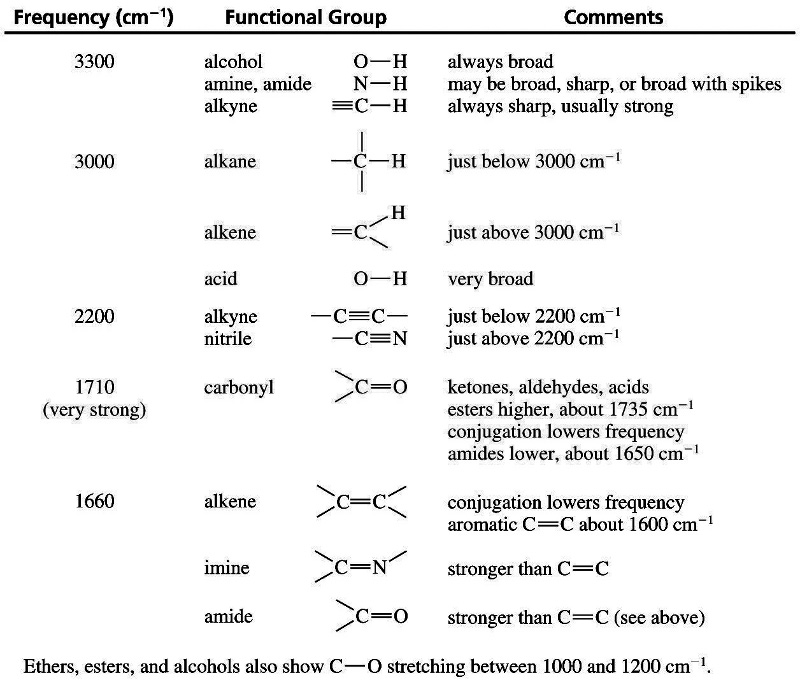
\includegraphics[width=12cm]{IR-Table}}
\end{figure}

\begin{figure}[h!]
	\centerline{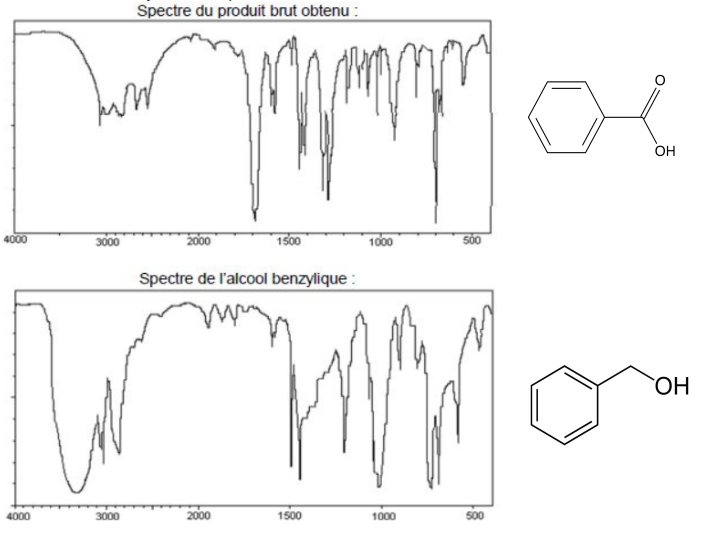
\includegraphics[width=16cm]{spectresIR}}
\end{figure}

\pagebreak


\newpage
\section{Spectroscopie à résonance magnétique nucléaire}
\subsection{Résonance magnétique nucléaire}
Attention sur cette partie à ne pas rater le placement : soit on fait bel et bien niveau lycée et on ne rentre PAS dans les explications, soit on prend le temps d'expliquer clairement sans dire de bêtises...Mais il ne faut pas faire un entre 2. \\

Cette méthode de spectroscopie s'intéresse au spin des noyaux atomiques en utilisant l'effet Zeeman. En effet tout comme les électrons les protons et neutrons qui composent les noyaux possèdent eux aussi un spin $\frac{1}{2}$ (car ce sont des bosons), les noyaux vont donc pouvoir avoir eux aussi un spin non nul, noté $I$. En l'occurrence il vaudra 0 si A et Z sont pairs, il sera entier si A est pair et Z impair et demi entier si A est impair. 
\paragraph{A ne pas dire} Le moment magnétique de spin $\vec{\mu} = \gamma \vec{L}$ va donner lieu à une énergie d'interaction $W_{mag} = -\vec{\mu}.\vec{B}$ lorsque l-on applique un champ extérieur $\vec{B}$. Si on prend un champ selon l'axe z, ce dernier va devenir l'axe de référence et on va donc avoir
\begin{eqnarray}
W = -\gamma L_z B \hspace{0.5cm} \mathrm{avec}\; \gamma = g\,\frac{q}{2m}
\end{eqnarray}
le facteur giromagnétique (et ou g est le facteur de Landé) sachant que le moment cinétique selon l'axe z est quantifié selon
\begin{eqnarray}
L_z | I,m\rangle = m\hbar |I ,m\rangle
\end{eqnarray}
on obtient comme énergies propres 
\begin{eqnarray}
W = -m_I\gamma \hbar B
\end{eqnarray}
et on aura ainsi $2I+1$ niveaux d'énergies disponibles.\\

Si on considère le cas le plus simple où le noyau possède un spin $\frac{1}{2}$ (noyau d'Hydrogène $^1_1H$ par exemple), on va, en appliquant un champ extérieur $\vec{B}$ créer deux niveaux d'énergie séparés par d'une énergie $\Delta E = \gamma \hbar B$. Par conséquent, si on envoie sur l'échantillon un photon d'énergie $h\nu$, il va être absorbé si 
\begin{eqnarray}
h\nu = \gamma \frac {h B}{2\pi},
\end{eqnarray}
les photons absorbés auront donc la fréquence 
\begin{eqnarray}
	\nu_0 = \frac{\gamma B}{2\pi}.
\end{eqnarray}
Si on trace l'absorbance en fonction de la fréquence envoyée on obtient donc des pics pour chaque atome de spin non nul présent dans l'échantillon. Afin d'avoir des spectres qui ne dépendent pas du champ $\vec{B}$ utilisé et donc de l'appareil utilisé, on définit une fréquence de référence correspondant à un pic connu et on trace le spectre en partie par million ou ppm défini comme 
\begin{eqnarray}
\delta = \frac{\nu-\nu_{ref}}{\nu_{ref}}.10^6.
\end{eqnarray}
\subsection{Déplacement chimique}
Dans la pratique on observe que pour une molécule possédant plusieurs atomes d'hydrogènes il peut se former différents pics situés à des fréquences distinctes. C'est dû à ce que l'on appelle le blindage : si il y a beaucoup d'électrons mobiles autour du proton considéré le champ magnétique va avoir plus de mal à interagir avec le proton et la fréquence de résonance sera ainsi plus faible, c'est ce décalage par rapport à la valeur attendue que l'on nomme déplacement chimique.\\

Les protons qui subissent le même blindage sont dit équivalents, pour une molécule simple des protons sont équivalents si ils sont portés par le même atome, ou si il existe une symétrie dans la molécule permettant de les identifier. Faire un schéma avec le 1-bromo-2,2-diméthylpropane
\begin{eqnarray}
&CH_3& \nonumber\\
&|& \nonumber \\
H_3C  &-\,C\,-&CH_2-Br\\
&|& \nonumber \\
&CH_3& \nonumber
\end{eqnarray}
 pour illustrer.\\
\begin{figure}[h]
	\centerline{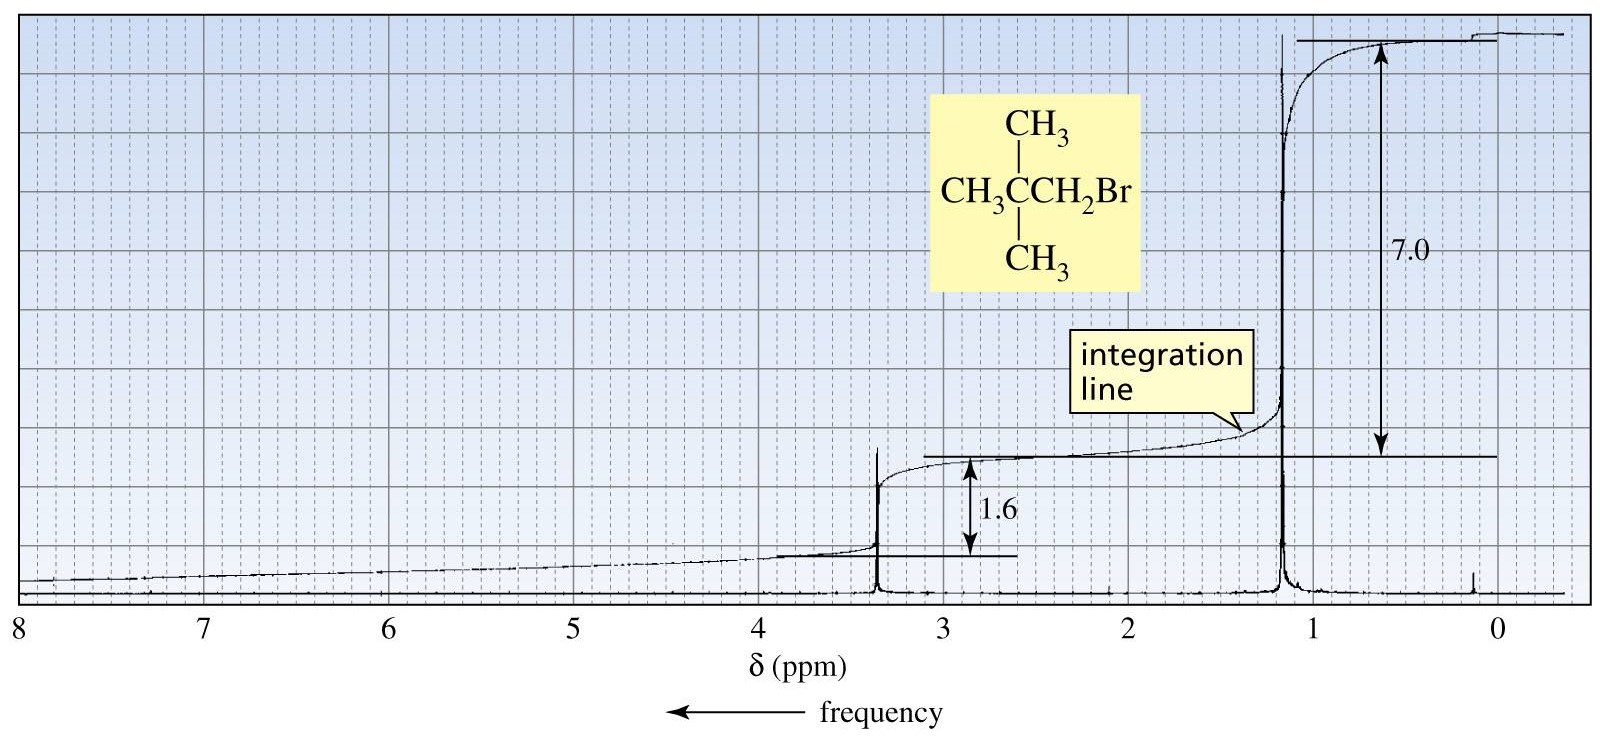
\includegraphics[width=14cm]{spectreRMN1}}
\end{figure}

Plus un l'atome portant les protons sera proche d'un atome électronégatif, plus il sera "déserté" par les électrons et plus le blindage sera par conséquent faible et ainsi plus la fréquence de résonance $\mu_{res}$ sera élevée. Illustrer sur le même exemple.\\

\subsection{Aire et multiplicité}
On peut notamment remarquer que l'aire d'un pic est proportionnelle au nombre de protons équivalents qui y correspondent, ce qui va permettre d'associer chaque pic au groupe de protons équivalents correspondants. Montrer encore sur le même exemple\\

On peut remarquer sur le spectre de l'éthanol $CH_3-CH_2-OH$ que deux des pics attendus sont "éparpillés" en petit pics secondaires.
\begin{figure}[h]
	\centerline{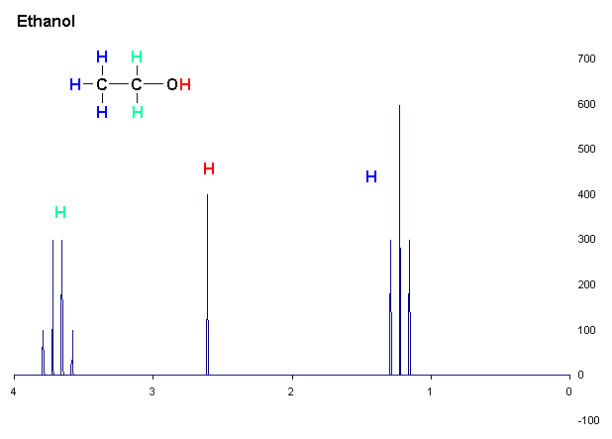
\includegraphics[width=13cm]{RMN2_0}}
\end{figure}
Cela s'explique par des interactions spin-spin entre protons voisins non équivalents, ce qu'il faut retenir c'est que si un groupement de proton portés par un atome, voit n autres protons portés par l'atome voisin, alors le pic associé à ce groupe sera un n+1uplet.

\subsection{Application}
Via tous les aspects décrits ici, on est en mesure d'associer un spectre simple à la molécule qui y correspond, notamment pour une molécule proche de l'acide benzoïque synthétisé précédemment.
\begin{figure}
	\centerline{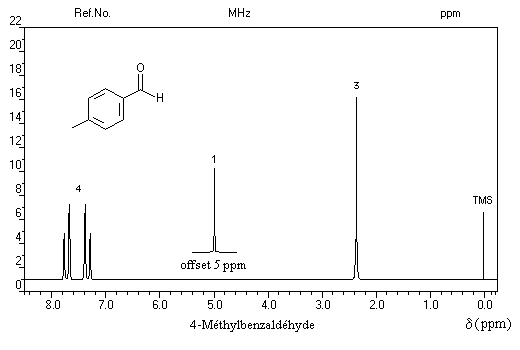
\includegraphics[width=14cm]{RMN3}}
\end{figure}
 Dans la pratique la RMN est la technique par excellence utilisée en chimie organique pour déterminer la structure d'une molécule.

\section{Conclusion}
On a vu dans cette leçon que les diverses techniques de spectroscopie permettent de déterminer avec une remarquable précision la structure de molécules organiques.

\section*{Remarques}
Regarder la spectroscopie Raman pour les questions.\\
Mettre en valeur le fait que ces méthodes de caractérisation sont non destructives.\\
Mettre du lien entre les différentes parties et montrer que ces trois spectroscopies forment un ensemble permettant une bonne caractérisation en apportant chacune une partie du puzzle permettant de remonter à la structure de la molécule.\\
Pour les spectres possibilité d'utiliser le logiciel gratuit Specamp.\\
Possibilité de mener un calcul de rendement pour la synthèse de l'indigo pour montrer notre capacité à mener le calcul.
\subsubsection{Bibliographie recommandée}
Atkins Chimie-Physique\\
Vollhardt\\
Clayden



\end{document}